% ថ្នាក់ទី ១១ (វិទ្យាសាស្ត្រសង្គម) · ជំពូកទី ១ ស៊ីត · មេរៀនទី ១ · សៀវភៅ ទំព័រ ១–៧
\chapter{ស៊ីតចំនួនពិត}

\begin{note}[ជំពូកទី ១ ៖ ស៊ីត]
ជំពូកនេះមានមេរៀន ៖ \textbf{១. ស៊ីតចំនួនពិត} \quad \textbf{២. ស៊ីតនព្វន្ត} \quad \textbf{៣. ស៊ីតធរណីមាត្រ} ។

ការសិក្សាស៊ីត គឺបណ្ដាលឱ្យគណិតវិទ្យាកាន់តែមានការរីកចម្រើនឡើងពីមួយថ្ងៃទៅមួយថ្ងៃ តាមរយៈផលបូកតួនៃស៊ីតអាចឱ្យគេសង់បាននូវតារាងនៃអនុគមន៍ត្រីកោណមាត្រ និងអនុគមន៍លោការីតមិនត្រឹមតែប៉ុណ្ណោះក៏អាចឱ្យគេគណនាបាននូវតម្លៃលេខ $e$ និង $\pi$ ទៀតផង ។
\[
e = 1 + \frac{1}{1!} + \frac{1}{2!} + \frac{1}{3!} + \frac{1}{4!} + \frac{1}{5!} + \frac{1}{6!} + \frac{1}{7!} + \dots
\]
\[
\frac{\pi}{4} = 1 - \frac{1}{3} + \frac{1}{5} - \frac{1}{7} + \frac{1}{9} - \frac{1}{11} + \frac{1}{13} - \frac{1}{15} + \dots
\]
\end{note}

\begin{objBox}[វត្ថុបំណង]
\begin{enumerate}[1]
  \item បង្ហាញសញ្ញាណស៊ីតចំនួនពិត ស៊ីតរាប់អស់ និងស៊ីតអនន្តតួ
  \item សរសេរតួនៃស៊ីតនិងកំណត់តួទី $n$ នៃស៊ីត
  \item បង្ហាញថាស៊ីតមួយជាស៊ីតកើនឬស៊ីតចុះ
  \item បង្ហាញស៊ីតម៉ូណូតូន ។
\end{enumerate}
\end{objBox}

\section{សញ្ញាណស៊ីត}

\begin{example}[ឧទាហរណ៍ ១]
គេមានចំនួនគត់ធម្មជាតិ $1, 2, 3, 4, 5, \ldots$ ។\\
គេមានចំនួនគត់គូ $2, 4, 6, 8, 10, \ldots$ ។\\
គេមានចំនួនគត់សេសតូចជាង $16$ គឺ $1, 3, 5, 7, 9, 11, 13, 15$ ។\\
គេមានចំនួនសនិទាន $1, \frac{1}{2}, \frac{1}{3}, \frac{1}{4}, \frac{1}{5}, \frac{1}{6}$ ។
\end{example}

ចំនួនដែលរៀបតាមលំដាប់នេះហៅថា \textbf{ស៊ីតនៃចំនួនពិត} ។ ស៊ីតនៃចំនួនពិត $1, 2, 3, 4, 5, \ldots$ ហៅថា \textbf{ស៊ីតអនន្តតួ} ។ ស៊ីតអនន្តតួ គឺជាស៊ីតដែលមានចំនួនតួច្រើនរាប់មិនអស់ ។

ម្យ៉ាងទៀត ស៊ីតនៃចំនួនពិត $1, 3, 5, 7, 9, 11, 13, 15$ និងស៊ីតនៃចំនួនសនិទាន $1, \frac{1}{2}, \frac{1}{3}, \frac{1}{4}, \frac{1}{5}, \frac{1}{6}$ ហៅថា \textbf{ស៊ីតរាប់អស់} ។ ស៊ីតរាប់អស់គឺជាស៊ីតដែលគេរាប់ចំនួនតួបាន ។ ក្នុងស៊ីតរាប់អស់គេអាចស្គាល់ចំនួនតួនិងតួចុងក្រោយនៃស៊ីត ។

\begin{example}[ឧទាហរណ៍ ២]
គេមានអនុគមន៍ $f : \mathbb{N} \to \mathbb{R}$, $n \mapsto f(n) = 2n + 1$ គេសង្កេតឃើញថា
\[
\begin{aligned}
&\text{បើ } n = 1 \text{ នោះ } f(1) = 2 \times 1 + 1 = 3\\
&\text{បើ } n = 2 \text{ នោះ } f(2) = 2 \times 2 + 1 = 5\\
&\text{បើ } n = 3 \text{ នោះ } f(3) = 2 \times 3 + 1 = 7\\
&\text{បើ } n = 4 \text{ នោះ } f(4) = 2 \times 4 + 1 = 9\\
&\ldots\ldots
\end{aligned}
\]
គេបានចំនួនរៀបតាមលំដាប់ $3, 5, 7, 9, \ldots$ បង្កើតបានជាស៊ីតនៃចំនួនពិត ។ ចំនួននីមួយៗនៃស៊ីតហៅថា \textbf{តួ} ។ ចំនួន $3$ ហៅថាតួទី $1$, $5$ តួទី $2$, $7$ តួទី $3$ \ldots រៀងគ្នា ។
\end{example}

\begin{definition}
ស៊ីតចំនួនពិតគឺជាអនុគមន៍លេខដែលកំណត់ពី $\mathbb{N}$ ទៅ $\mathbb{R}$ ។
\end{definition}

ជាទូទៅគេប្រើអក្សរ $a_1, a_2, a_3, \ldots, a_n$ សម្រាប់តាងឱ្យតួនៃស៊ីតដែល $a_1$ ជាតួទី $1$, $a_2$ ជាតួទី $2$, $\ldots$, $a_n$ ជាតួទី $n$ ។

គេតាងស៊ីតនោះដោយនិមិត្តសញ្ញា $(a_n)$ ដែល $n \in \mathbb{N}$, $\mathbb{N} = \{1, 2, 3, \ldots\}$ ។

\begin{example}[លំហាត់គំរូ ១]
បំពេញតួនៃស៊ីតខាងក្រោមនេះឱ្យបានបីតួទៀត
\begin{enumerate}[a]
  \item $1, 5, 9, \ldots$
  \item $1, 8, 27, \ldots$
\end{enumerate}
\end{example}
\ans
\begin{enumerate}[a]
  \item $1, 5, 9, 13, 17, 21$
  \item $1, 8, 27, 64, 125, 216$ ។
\end{enumerate}

\begin{example}[លំហាត់គំរូ ២]
សរសេរគ្រប់តួនៃស៊ីតរាប់អស់ $a_n = \dfrac{(-1)^{n+1}}{n+1}$, $1 \le n \le 5$ ។
\end{example}
\ans
ជំនួសចំនួនគត់ធម្មជាតិពី $1$ ដល់ $5$ ក្នុង $a_n$ ។ គេបាន
\[
\begin{gathered} a_1 = \frac{(-1)^2}{2} = \frac{1}{2},\quad a_2 = \frac{(-1)^3}{3} = -\frac{1}{3},\\ a_3 = \frac{(-1)^4}{4} = \frac{1}{4},\quad a_4 = \frac{(-1)^5}{5} = -\frac{1}{5} \end{gathered}
\]
\[
a_5 = \frac{(-1)^6}{6} = \frac{1}{6}
\]
ដូច្នេះប្រាំតួនៃស៊ីតគឺ $\frac{1}{2}, -\frac{1}{3}, \frac{1}{4}, -\frac{1}{5}, \frac{1}{6}$ ។

\begin{pro}
\begin{enumerate}[a]
  \item គេឱ្យស៊ីត $3, 8, 15, \ldots$ ។ បន្តសរសេរស៊ីតនេះឱ្យបានបីតួទៀត ។
  \item សរសេរតួនៃស៊ីត $(a_n)$ កំណត់ដោយ $a_n = \dfrac{1}{n+2}$ ដែល $1 \le n \le 4$ ។
  \item សរសេរតួនៃស៊ីតតាមលំដាប់តគ្នា $a_n = 2 + \dfrac{1}{2^n}$ ដែល $n \in \mathbb{N}$ ។
\end{enumerate}
\ans
\begin{enumerate}[a]
  \item $24, 35, 48$
  \item $\frac{1}{3}, \frac{1}{4}, \frac{1}{5}, \frac{1}{6}$
  \item $\frac{5}{2}, \frac{9}{4}, \frac{17}{8}, \ldots, 2 + \frac{1}{2^n}$ ។
\end{enumerate}
\end{pro}

\section{តួទី \texorpdfstring{$n$}{n} នៃស៊ីត}

\begin{example}[ឧទាហរណ៍ ១]
គេឱ្យស៊ីតចំនួនគត់ $1, 2, 3, 4, 5, \ldots$ ដែលតួចុងក្រោយរបស់វាតាងដោយ $n$ ។ ក្នុងករណីគេថា $a_1 = 1$ ជាតួទី $1$, $a_2 = 2$ ជាតួទី $2$, $a_3 = 3$ ជាតួទី $3$, $\ldots$, $a_n = n$ ជាតួទី $n$ ។
\end{example}

\begin{example}[ឧទាហរណ៍ ២]
ចំពោះស៊ីតនៃចំនួន $2, 4, 6, 8, 10, \ldots$ ។ គេឃើញថា
\[
\begin{gathered} a_1 = 2 = 2 \times 1,\quad a_2 = 4 = 2 \times 2,\quad a_3 = 6 = 2 \times 3,\\ a_4 = 8 = 2 \times 4,\ \ldots,\ a_n = 2 \times n \end{gathered}
\]
ដូច្នេះ គេបានតួទី $n$ នៃស៊ីតគឺ $a_n = 2 \times n$ ។
\end{example}

តាមឧទាហរណ៍ខាងលើ បើគេស្គាល់តួដំបូង និងតួបន្តបន្ទាប់នៃស៊ីត ដើម្បីសរសេររូបមន្តតួទី $n$ នៃស៊ីតគេពិនិត្យមើលតួនីមួយៗនៃស៊ីត រួចរកមើលលំនាំគំរូរបស់វា ។ តួនីមួយៗជាអនុគមន៍នៃចំនួនតួ ។ តួទី $1$ ត្រូវនឹង $n = 1$ តួទី $2$ ត្រូវនឹង $n = 2$, $\ldots$, តួទី $n$ ត្រូវនឹង $n = n$ ។

\begin{example}[លំហាត់គំរូ ១]
កំណត់តួទី $n$ នៃស៊ីត $3, 5, 7, 11, \ldots$ ចំពោះគ្រប់ $n \in \mathbb{N}$ ។
\end{example}
\ans
គេសង្កេតឃើញថា
\[
\begin{aligned}
a_1 &= 3 = 2 \times 1 + 1\\
a_2 &= 5 = 2 \times 2 + 1\\
a_3 &= 7 = 2 \times 3 + 1\\
a_4 &= 9 = 2 \times 4 + 1\\
a_5 &= 11 = 2 \times 5 + 1\\
&\ \,\vdots\\
a_n &= 2n + 1
\end{aligned}
\]
ដូច្នេះគេបានតួទី $n$ នៃស៊ីត $a_n = 2n + 1$ ។

\begin{example}[លំហាត់គំរូ ២]
បាល់មួយត្រូវបានទម្លាក់ពីកម្ពស់ $6\text{ m}$ ។ ដោយដឹងថា បាល់នោះធ្លាក់ដល់ដីតែងតែលោតឡើងលើវិញបាន $\frac{2}{3}$ នៃកម្ពស់ដែលបាល់នោះធ្លាក់ចុះ ។ ចូរកំណត់កម្ពស់ នៃបាល់ជាបន្តបន្ទាប់ដោយសរសេរជាស៊ីតមួយ រួចកំណត់តួទី $n$ នៃស៊ីតនេះ ។

\begin{center}
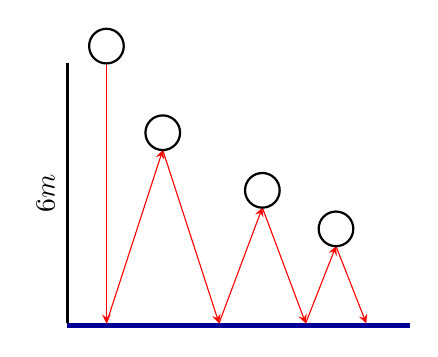
\begin{tikzpicture}[scale=0.55,>=stealth]
  \fill[blue!60!black] (-0.3,-0.12) rectangle (7.6,0);
  \draw[thick] (-0.3,0) -- (-0.3,6);
  \node[rotate=90] at (-0.8,3) {$6\text{ m}$};
  \draw[red,->] (0.6,6) -- (0.6,0);
  \draw[red,->] (0.6,0) -- (1.9,4);
  \draw[red,->] (1.9,4) -- (3.2,0);
  \draw[red,->] (3.2,0) -- (4.2,2.67);
  \draw[red,->] (4.2,2.67) -- (5.2,0);
  \draw[red,->] (5.2,0) -- (5.9,1.78);
  \draw[red,->] (5.9,1.78) -- (6.6,0);
  \foreach \x/\y in {0.6/6, 1.9/4, 4.2/2.67, 5.9/1.78}
    \draw[fill=white,thick] (\x,\y+0.4) circle (0.4);
\end{tikzpicture}
\end{center}
\end{example}
\ans
លើកដំបូងបាល់ធ្លាក់ពីកម្ពស់ $6\text{ m}$ ដូចបង្ហាញក្នុងរូប រួចលោតឡើងលើវិញបាន $\frac{2}{3}$ នៃ $6\text{ m}$ ឬ $6\left(\frac{2}{3}\right)\text{ m}$ មានកម្ពស់ $4\text{ m}$ ។ លើកទី $2$ បាល់ធ្លាក់ពីកម្ពស់ $6\left(\frac{2}{3}\right)\text{ m}$ ហើយលោតឡើងលើវិញបាន $6\left(\frac{2}{3}\right)\left(\frac{2}{3}\right)$ ឬ $6\left(\frac{2}{3}\right)^2$ ។

ដូច្នេះ កម្ពស់បាល់ជាបន្តបន្ទាប់គឺ
\[
6 \times \left(\frac{2}{3}\right)^1,\ 6 \times \left(\frac{2}{3}\right)^2,\ 6 \times \left(\frac{2}{3}\right)^3,\ 6 \times \left(\frac{2}{3}\right)^4,\ \ldots
\]
ហើយតួទី $n$ គឺ $a_n = 6 \times \left(\dfrac{2}{3}\right)^{n-1}$ ។

\begin{pro}
កំណត់តួទី $n$ ចំពោះ គ្រប់ $n \in \mathbb{N}$ នៃស៊ីតខាងក្រោម ៖
\begin{enumerate}[a]
  \item $-1, 2, 7, 14, 23, \ldots$
  \item $\frac{2}{3}, \frac{3}{4}, \frac{4}{5}, \frac{5}{6}, \ldots$ ។
\end{enumerate}
\ans
\begin{enumerate}[a]
  \item $a_n = n^2 - 2$
  \item $a_n = \dfrac{n+1}{n+2}$ ។
\end{enumerate}
\end{pro}

\section{អថេរភាពនៃស៊ីត}
\subsection{ស៊ីតកើន ស៊ីតចុះ}

\begin{example}[ឧទាហរណ៍ ១]
គេឱ្យស៊ីត $(a_n)_{n \in \mathbb{N}}$ ដែល $a_n = n$ ។

គេបានតួនៃស៊ីតគឺ $1, 2, 3, 4, \ldots, n$ ។ តាមលំដាប់តួនៃស៊ីត គេសង្កេតឃើញថា $1 < 2 < 3 < 4 < 5 < \ldots$ ឬ $a_1 < a_2 < a_3 < \ldots < a_n < a_{n+1} < \ldots$ នោះគេបានស៊ីត $(a_n)$ ហៅថាស៊ីតកើនដាច់ខាត ។
\end{example}

\begin{example}[ឧទាហរណ៍ ២]
គេឱ្យស៊ីត $(a_n)_{n \in \mathbb{N}}$ ដែលមានតួ $1, 1, 2, 3, 4, 5, \ldots$ ឬ $a_1 \le a_2 \le a_3 \le \ldots \le a_n \le a_{n+1} \le \ldots$ នោះគេបានស៊ីត $(a_n)$ ហៅថាស៊ីតកើន ។
\end{example}

\begin{example}[ឧទាហរណ៍ ៣]
គេឱ្យស៊ីត $(a_n)_{n \in \mathbb{N}}$ ដែល $a_n = \dfrac{1}{n}$ ។

គេបានតួនៃស៊ីតគឺ $1, \frac{1}{2}, \frac{1}{3}, \frac{1}{4}, \frac{1}{5}, \ldots$ ។ តាមលំដាប់តួនៃស៊ីត គេសង្កេតឃើញថា $1 > \frac{1}{2} > \frac{1}{3} > \frac{1}{4} > \frac{1}{5}, \ldots$ ឬ $a_1 > a_2 > a_3 > \ldots > a_n > a_{n+1} > \ldots$ ឬ $a_1 \ge a_2 \ge a_3 \ge \ldots \ge a_n \ge a_{n+1} \ge \ldots$ នោះគេបានស៊ីត $(a_n)$ ហៅថាស៊ីតចុះ ។
\end{example}

\begin{definition}
\begin{itemize}
  \item ស៊ីត $(a_n)$ ជាស៊ីតកើន លុះត្រាតែចំពោះគ្រប់ចំនួនគត់ធម្មជាតិ $n \in \mathbb{N}$, $a_{n+1} \ge a_n$ ។
  \item ស៊ីត $(a_n)$ ជាស៊ីតចុះ លុះត្រាតែចំពោះគ្រប់ចំនួនគត់ធម្មជាតិ $n \in \mathbb{N}$, $a_{n+1} \le a_n$ ។
\end{itemize}
\end{definition}

\begin{example}[លំហាត់គំរូ]
\begin{enumerate}[a]
  \item បង្ហាញថាស៊ីត $(a_n)$ ដែល $a_n = 3n + 1$ ជាស៊ីតកើន ។
  \item បង្ហាញថាស៊ីត $(b_n)$ ដែល $b_n = 12 - 2n$ ជាស៊ីតចុះ ។
\end{enumerate}
\end{example}
\ans
\begin{enumerate}[a]
  \item គេមាន $a_n = 3n + 1$, $a_{n+1} = 3(n+1) + 1 = 3n + 4$\\
  នោះគេបាន $a_{n+1} - a_n = 3n + 4 - (3n + 1) = 3 > 0$ នាំឱ្យ $a_{n+1} > a_n$ ។\\
  ដូច្នេះ ស៊ីត $(a_n)$ ដែល $a_n = 3n + 1$ ជាស៊ីតកើន ។
  \item គេមាន $b_n = 12 - 2n$, $b_{n+1} = 12 - 2(n+1) = 10 - 2n$\\
  នោះគេបាន $b_{n+1} - b_n = 10 - 2n - (12 - 2n) = -2 < 0$ នាំឱ្យ $b_{n+1} < b_n$ ។\\
  ដូច្នេះ ស៊ីត $(b_n)$ ដែល $b_n = 12 - 2n$ ជាស៊ីតចុះ ។
\end{enumerate}

\begin{pro}
តើស៊ីតខាងក្រោមមួយណាជាស៊ីតកើន មួយណាជាស៊ីតចុះ ។
\begin{enumerate}[a]
  \item ស៊ីត $(a_n)_{n \ge 5}$ ដែល $a_n = \dfrac{3n}{2}$
  \item ស៊ីត $(a_n)_{n \ge 3}$ ដែល $a_n = \dfrac{2}{n}$ ។
\end{enumerate}
\ans
\begin{enumerate}[a]
  \item ស៊ីត $(a_n)$ ជាស៊ីតកើន
  \item ស៊ីត $(a_n)$ ជាស៊ីតចុះ ។
\end{enumerate}
\end{pro}

\subsection{ស៊ីតម៉ូណូតូន}

\begin{example}[ឧទាហរណ៍ ១]
គេឱ្យស៊ីត $(a_n)_{n \in \mathbb{N}}$ ដែល $a_n = \dfrac{n}{n+1}$ ។

គេបានតួនៃស៊ីតគឺ $\frac{1}{2}, \frac{2}{3}, \frac{3}{4}, \frac{4}{5}, \ldots$ ។ តាមលំដាប់តួនៃស៊ីត គេសង្កេតឃើញថា $\frac{1}{2} < \frac{2}{3} < \frac{3}{4} < \frac{4}{5} < \ldots$ ឬ $a_1 < a_2 < a_3 < a_4 < \ldots < a_n < a_{n+1} < \ldots$ ។

ដូច្នេះ ស៊ីត $(a_n)$ ជាស៊ីតកើន នោះគេថាស៊ីត $(a_n)_{n \in \mathbb{N}}$ នេះជាស៊ីតម៉ូណូតូន ។
\end{example}

\begin{example}[ឧទាហរណ៍ ២]
គេឱ្យស៊ីត $(a_n)_{n \in \mathbb{N}}$ ដែល $a_n = 1 + \dfrac{1}{n}$ ។

គេបានតួនៃស៊ីតគឺ $2, \frac{3}{2}, \frac{4}{3}, \frac{5}{4}, \ldots$ ។ តាមលំដាប់តួនៃស៊ីត គេសង្កេតឃើញថា $2 > \frac{3}{2} > \frac{4}{3} > \frac{5}{4} > \ldots$ ឬ $a_1 > a_2 > a_3 > a_4 > \ldots > a_n > a_{n+1} > \ldots$ ។

ដូច្នេះ ស៊ីត $(a_n)$ ជាស៊ីតចុះ នោះគេថាស៊ីតនេះជា \textbf{ស៊ីតម៉ូណូតូន} ។
\end{example}

\begin{definition}
ស៊ីត $(a_n)$ ជាស៊ីតម៉ូណូតូន កាលណាស៊ីត $(a_n)$ ជាស៊ីតកើនឬជាស៊ីតចុះ ។
\end{definition}

\begin{example}[លំហាត់គំរូ]
បង្ហាញថាស៊ីត $(a_n)_{n \in \mathbb{N}}$ ជាស៊ីតម៉ូណូតូន $a_n = \dfrac{n}{n+1}$ ។
\end{example}
\ans
\textbf{របៀបទី ១} ៖ គេមាន $a_n = \dfrac{n}{n+1}$ គេបាន $a_{n+1} = \dfrac{n+1}{(n+1)+1} = \dfrac{n+1}{n+2}$ ។

ចំពោះ $\forall n \ge 1$ គេបាន
\[
\begin{aligned} a_{n+1} - a_n &= \frac{n+1}{n+2} - \frac{n}{n+1} = \frac{(n+1)^2 - n(n+2)}{(n+2)(n+1)}\\ &= \frac{1}{(n+1)(n+2)} > 0 \end{aligned}
\]
នោះ $a_{n+1} > a_n$ ដូច្នេះ ស៊ីត $(a_n)_{n \in \mathbb{N}}$ ជាស៊ីតម៉ូណូតូន ។

\textbf{របៀបទី ២} ៖ ដោយ $a_n = \dfrac{n}{n+1} > 0$, $\forall n \in \mathbb{N}$ គេបាន
\[
a_{n+1} = \frac{n+1}{(n+1)+1} = \frac{n+1}{n+2} > 0,\quad \forall n \in \mathbb{N}
\]
\[
\frac{a_{n+1}}{a_n} = \frac{\dfrac{n+1}{n+2}}{\dfrac{n}{n+1}} = \frac{n+1}{n+2} \times \frac{n+1}{n} = \frac{n^2 + 2n + 1}{n^2 + 2n} > 1
\]
ព្រោះ $\forall n \ge 1$ ឬ $n^2 + 2n + 1 > n^2 + 2n$ នោះ $a_{n+1} > a_n$ ។

ដូច្នេះ ស៊ីត $(a_n)_{n \in \mathbb{N}}$ ជាស៊ីតម៉ូណូតូន ។

\begin{pro}
តើស៊ីតខាងក្រោម ស៊ីតណាជាស៊ីតម៉ូណូតូន ។
\begin{enumerate}[a]
  \item $1, \frac{1}{2}, \frac{1}{3}, \frac{1}{4}, \frac{1}{5}, \ldots, \frac{1}{n}, \ldots$
  \item $a_n = \dfrac{2^n}{n}$, $n \ge 1$
  \item $1, -\frac{1}{2}, \frac{1}{3}, -\frac{1}{4}, \ldots, (-1)^{n+1}\frac{1}{n}, \ldots$
\end{enumerate}
\ans
\begin{enumerate}[a]
  \item $1, \frac{1}{2}, \frac{1}{3}, \frac{1}{4}, \frac{1}{5}, \ldots, \frac{1}{n}, \ldots$ ជាស៊ីតម៉ូណូតូន
  \item $(a_n)$ ជាស៊ីតម៉ូណូតូន
  \item $1, -\frac{1}{2}, \frac{1}{3}, -\frac{1}{4}, \ldots, (-1)^{n+1} \times \frac{1}{n}$ មិនមែនជាស៊ីតម៉ូណូតូន ។
\end{enumerate}
\end{pro}

\section*{លំហាត់អនុវត្តន៍}
\begin{enumerate}[1]
  \item សរសេរបីតួបន្ទាប់នៃស៊ីតខាងក្រោម ៖
  \begin{tasks}(2)
    \task $5, 10, 15, 20, \ldots$
    \task $1, 5, 14, 30, 55, \ldots$ ។
  \end{tasks}
  \item សរសេរតួនៃស៊ីតរាប់អស់ខាងក្រោម ៖
  \begin{tasks}(2)
    \task $a_n = \dfrac{(-1)^n}{n}$ ចំពោះ $1 \le n \le 8$
    \task $b_n = (2)^{-n+2}$ ចំពោះ $1 \le n \le 5$ ។
  \end{tasks}
  \item សរសេរបួនតួដំបូងនៃស៊ីតរាប់អស់ខាងក្រោម ៖
  \begin{tasks}(4)
    \task $a_n = \dfrac{(-1)^n}{n^2}$
    \task $b_n = \dfrac{1}{n^2 + n}$
    \task $c_n = (-1)^n (n-2)^2$
    \task $d_n = (-1)^n 2^{n-1}$ ។
  \end{tasks}
  \item កំណត់តួទី $n$ ចំពោះគ្រប់ $n \in \mathbb{N}$ នៃស៊ីតខាងក្រោម ៖
  \begin{tasks}(4)
    \task $5, 7, 9, 11, 13, \ldots$
    \task $-3, -1, 1, 3, 5, \ldots$
    \task $16, 13, 10, 7, 4, \ldots$
    \task $\frac{2}{3}, \frac{3}{5}, \frac{4}{7}, \frac{5}{9}, \ldots$ ។
  \end{tasks}
  \item បង្ហាញថាស៊ីត $(a_n)$ ដែល $a_n = \dfrac{1}{n+3}$ ជាស៊ីតចុះ ។
  \item បង្ហាញថាស៊ីត $(b_n)$ ដែល $b_n = \dfrac{2n+1}{n+3}$ ជាស៊ីតកើន ។
  \item សិក្សាភាពម៉ូណូតូននៃស៊ីតដែលកំណត់ដូចខាងក្រោម ៖
  \begin{enumerate}[a]
    \item ស៊ីត $(a_n)_{n \in \mathbb{N}}$ ដែល $a_n = \dfrac{1}{n}$
    \item ស៊ីត $(a_n)$ ដែល $a_n = n^3 + 4n - 5$
    \item ស៊ីត $(a_n)$ ដែល $a_{n+1} = a_n^2$ និង $a_1 = 2$ ។
  \end{enumerate}
  \item គេមានស៊ីត $(a_n)$ ដែល $n$ ជាចំនួនគត់ធម្មជាតិ ហើយ $a_1 = 1$ និង $a_{n+1} = a_n^2 + a_n + 1$ ។
  \begin{enumerate}[a]
    \item បង្ហាញថាស៊ីត $(a_n)$ ដែល $n$ ជាចំនួនគត់ធម្មជាតិ ជាស៊ីតកើន ។
    \item បង្ហាញថាចំពោះគ្រប់ $n$, $a_n \ge n$ ។
  \end{enumerate}
\end{enumerate}
